\documentclass[12pt]{article}

% Math package
% leqno means numbered equations are displayed with the numbers to the left of
% the equations instead of to the right ("left equation numbers")
\usepackage[leqno]{amsmath}

% Geometry package for setting margins
\usepackage{geometry}
% Set margins
\geometry{margin=1in}

% Package for sans-serif font
\usepackage{helvet}
\renewcommand{\familydefault}{\sfdefault}

% Package for adding space between paragraphs
\usepackage{parskip}

% Adding "Page {number} of {total}" in footer
\usepackage{lastpage}
\usepackage{fancyhdr}
\fancyfoot[C]{Page \thepage\ of {\hypersetup{linkcolor=black}\pageref{LastPage}}}
\pagestyle{fancy}
% Remove horizontal line from header
\renewcommand{\headrulewidth}{0pt}

% Floating images
\usepackage{float}

% Subfigure images
\usepackage{subcaption}

% Making the "Figure #" bold in figures
\usepackage[labelfont=bf]{caption}

% Hyperlinks
\usepackage{hyperref}
\hypersetup{
    colorlinks,
    citecolor=black
}

% Referencing sections and include their name in the reference
\usepackage{nameref}

% Fill table of contents lines with dots
\usepackage{tocloft}
\renewcommand{\cftsecleader}{\cftdotfill{\cftdotsep}}

% Appendix package
\usepackage[title, titletoc]{appendix}

% Package for including other PDFs in this report
\usepackage{pdfpages}

% Bibliography
% \usepackage{natbib}
% \bibliographystyle{ieeetr}
% \bibliography{references}

\usepackage{etoolbox} % Required for patching commands
% Patch \bibliography to remove the "References" section title
\makeatletter
\patchcmd{\thebibliography}{\section*{\refname}}{}{}{}
\makeatother

% User requirement counter
\newcounter{mycounter}
\newcommand\showmycounter{\addtocounter{mycounter}{1}\ifnum\value{mycounter}<10 0\fi\themycounter}

\begin{document}

    \newgeometry{left=1.3in, right=1.3in}
    \newlength\myheight
    \newlength\mydepth
    \settototalheight\myheight{Xygp}
    \settodepth\mydepth{Xygp}
    \setlength\fboxsep{0pt}
    \setlength{\fboxrule}{0pt}
    \begin{titlepage}
        \Huge\textbf{EECS 4312 Software Requirements}

        \Large\textbf{Assignment 1}

        \Large Daniel Di Giovanni --- 218204818

        \large \today

        \vfill

        \normalsize
        \begin{center}
            \rule{\textwidth}{1pt}\\
        \end{center}

        \textbf{My signature below attests that this submission is my original work:}
            % Make sure this line is justified
            \unskip\parfillskip 0pt \par

        \small
        Following professional engineering practice, I bear the burden of
            proof for original work. I have read the
            \href{https://www.yorku.ca/secretariat/policies/policies/academic-honesty-senate-policy-on/}{Senate Policy on Academic Integrity posted on the York University website}
            and confirm that this work is in accordance with the Policy.
        \vspace*{0.5cm}
        \noindent

        \begin{center}
            \begin{tabular}{ll}
                \raisebox{-30pt}{\fbox{
\includegraphics[height=30pt]{images/signature.jpeg}}} & \raisebox{-30pt}{\fbox{\today}}\\
                \makebox[2.5in]{\hrulefill} & \makebox[2.5in]{\hrulefill}\\
                \textbf{Signature} & \textbf{Date}\\
            \end{tabular}
        \end{center}
    \end{titlepage}

    \setlength\fboxsep{5pt}
    \setlength{\fboxrule}{1pt}
    \restoregeometry

    \markboth{}{}
    {\hypersetup{linkcolor=black}
        \tableofcontents
        \thispagestyle{fancy}
    }
    \markboth{}{}

    \pagebreak

    \part*{Task 1: Choosing a Mobile App}
\addcontentsline{toc}{part}{Task 1: Choosing a Mobile App}

Loneliness in aging populations is an important issue, especially in Canada.

\section*{Introduction and Background}
\addcontentsline{toc}{section}{Introduction and Background}

The well-being of the elderly population is strongly correlated to the quality
    of their social lives.
Loneliness substantially increases the risk of depression, mood disorders, and
    feelings of hopelessness in the elderly \cite{golden}.
This problem is especially daunting in Canada, where, according to estimates by
    the Government of Canada, 40\% of Canadian adults will be seniors by 2038
    \cite{canada}.

Many apps exist that aim to fulfill the need of maintaining social connections
    and staying in contact with friends and family.
Out of these apps and services, GrandPad stands out in its ability to meet user
    needs.

\section*{GrandPad}
\addcontentsline{toc}{section}{GrandPad}

GrandPad
    (Google Play ID
    \href
        {https://play.google.com/store/apps/details?id=net.grandpad.puma&hl=en}
        {net.grandpad.puma})
    is an app used to maintain a private social network between loved ones,
    including a senior user who owns a GrandPad tablet.

The app's goals are to provide instant messaging and high-quality video-calling
    in real-time across the world with secure connections.
As a simple, no-frills service to stay connected with loved ones, WhatsApp
    Messenger provides an easy-to-use app that can be utilized to maintain
    social connections across geographical barriers.

GrandPad's goal is to provide a platform for maintaining the social network of a
    senior loved one.
The app, along with the GrandPad tablet for elderly users, provides a
    user-friendly interface for audio and video calls, messages, sharing of
    photos and videos, and online games.
As a simple, no-frills service to keep a network of family members and friends
    connected, GrandPad provides an easy-to-use app that can be utilized to
    maintain social connections across geographical barriers.

Research conducted on this topic found that the majority of GrandPad users found
    the platform easy to use and felt more connected from using it
    \cite{grandpad_feasability}.
GrandPad is especially promising when compared with modern social media services,
    whose newsfeed-style platforms have mixed results in fostering meaningful
    socialization \cite{longjing}.
Currently, GrandPad stands out to be a leading tool in the category of senior
    apps for maintaining social connections.


    \part*{Task 2: Identify User, Software, and System Requirements}
\addcontentsline{toc}{part}{Task 2: - Identify User, Software, and System Requirements}

The identification of user, software, and system requirements were scraped and
    analyzed from the Google Play Store, both from the app's description and its
    reviews.

\section*{Analyzing WhatsApp Messenger's Google Play Reviews}
\addcontentsline{toc}{section}{Analyzing WhatsApp Messenger's Google Play Reviews}

The following explanation of the analysis of WhatsApp Messenger's reviews is a
    summary of the Jupyter Notebook in Appendix \ref{sec:data_preprocessing}.

Using the
    \href{https://pypi.org/project/google-play-scraper/}{google-play-scraper}
    Python library, reviews were scraped from the Google Play Store.
Initially, 328,500 reviews were scraped, most of which were under 10 words.
This is shown in the histogram below.
\begin{figure}[H]
    \centering
    \includegraphics[width=0.75\textwidth]{data_preprocessing_files/data_preprocessing_9_0.png}
\end{figure}
To reduce the amount of data to analyze, all reviews under 10 words were
    removed.
Additional filters were applied, like removing non-English reviews with the
    \href{https://pypi.org/project/langdetect/}{langdetect} Python library.
The reviews were then split by their rating (5 stars: positive, 2-4 stars:
    mixed, 1 star: negative) and run through a
    \href
        {https://scikit-learn.org/dev/modules/generated/sklearn.decomposition.LatentDirichletAllocation.html}
        {Latent Dirichlet Allocation (LDA) algorithm from Scikit Learn}
    to identify important topics from each category of the reviews.

\subsection*{User Requirements from Negative Reviews}
\addcontentsline{toc}{subsection}{User Requirements from Negative Reviews}

The analysis of negative reviews led to some recurring topics, which included
    banning of accounts without warning,
    lack of support if a user's account was hacked,
    and the prevalence of scam messages.

\begin{description}
    \item[\textbf{USER-01}]
        The user should not be banned without first receiving a warning for a
            specific behavior.
    \item[\textbf{USER-02}]
        If a user's account is banned, the user should receive a thorough and
            transparent explanation of why the ban happened.
    \item[\textbf{USER-03}]
        The user needs to have protection against people hacking into their
            account.
    \item[\textbf{USER-04}]
        The user needs to have access to support in the event of someone hacking
            into their account.
    \item[\textbf{USER-05}]
        The user needs to have the option to block all messages from unknown
            accounts to prevent scam attempts.
\end{description}

\subsection*{User Requirements from Mixed Reviews}
\addcontentsline{toc}{subsection}{User Requirements from Mixed Reviews}

When analyzing the mixed reviews, some recurring topics were
    backups of chat history,
    and multi-factor authentication/verification steps.

\begin{description}
    \item[\textbf{USER-01}]
        The user needs to be able to choose which chats to backup.
    \item[\textbf{USER-02}]
        Upon a backup failure, the user needs to be informed why the backup
            failed so that they can take action to fix the issue.
    \item[\textbf{USER-03}]
        The user needs to reload chats from a backup file.
    \item[\textbf{USER-04}]
        The user needs to be able to enable multi-factor authentication.
    \item[\textbf{USER-05}]
        Upon a failure with multi-factor authentication, the user needs to be
            informed why the verification failed.
\end{description}

\subsection*{User Requirements from Positive Reviews}
\addcontentsline{toc}{subsection}{User Requirements from Positive Reviews}

When analyzing positive reviews, prominent topics that were found include
    video and voice calling,
    messaging,
    fast communication,
    easy-to-use interface,
    connecting friends and family,
    and connecting people across the world.

\begin{description}
    \item[\textbf{USER-06}]
        The user needs to conduct voice calls with one or more people, fast
            enough to have a conversation in real time.
    \item[\textbf{USER-07}]
        The user needs to conduct video calls with one or more people, fast
            enough to have a conversation in real time.
    \item[\textbf{USER-08}]
        Under a strong network connection, the user needs to be able to send and
            receive messages from one or more people in less than one minute.
    \item[\textbf{USER-09}]
        The user should not need to pay for the app when used for its basic
            functionalities of calling, messaging, and sharing content.
    \item[\textbf{USER-10}]
        The user should not be distracted by advertisements when using the app.
    \item[\textbf{USER-11}]
        The user needs to be able to connect with support personnel if they are
            having problems with the app that they cannot fix.
\end{description}


    \fancyhead{}

    \part*{References}
    \addcontentsline{toc}{part}{References}
    \begingroup
        \def\section*#1{}
        \bibliographystyle{IEEEtran}
        \bibliography{references}
    \endgroup

    \pagebreak

    \part*{Appendices}
    \addcontentsline{toc}{part}{Appendices}
        \begin{appendices}
            The following appendices contain the code that was referenced
                throughout this report.
            Appendix \ref{sec:reviews_processing_notebook} contains the Jupyter
                Notebook for the data preprocessing of the WhatsApp Messenger
                reviews.

            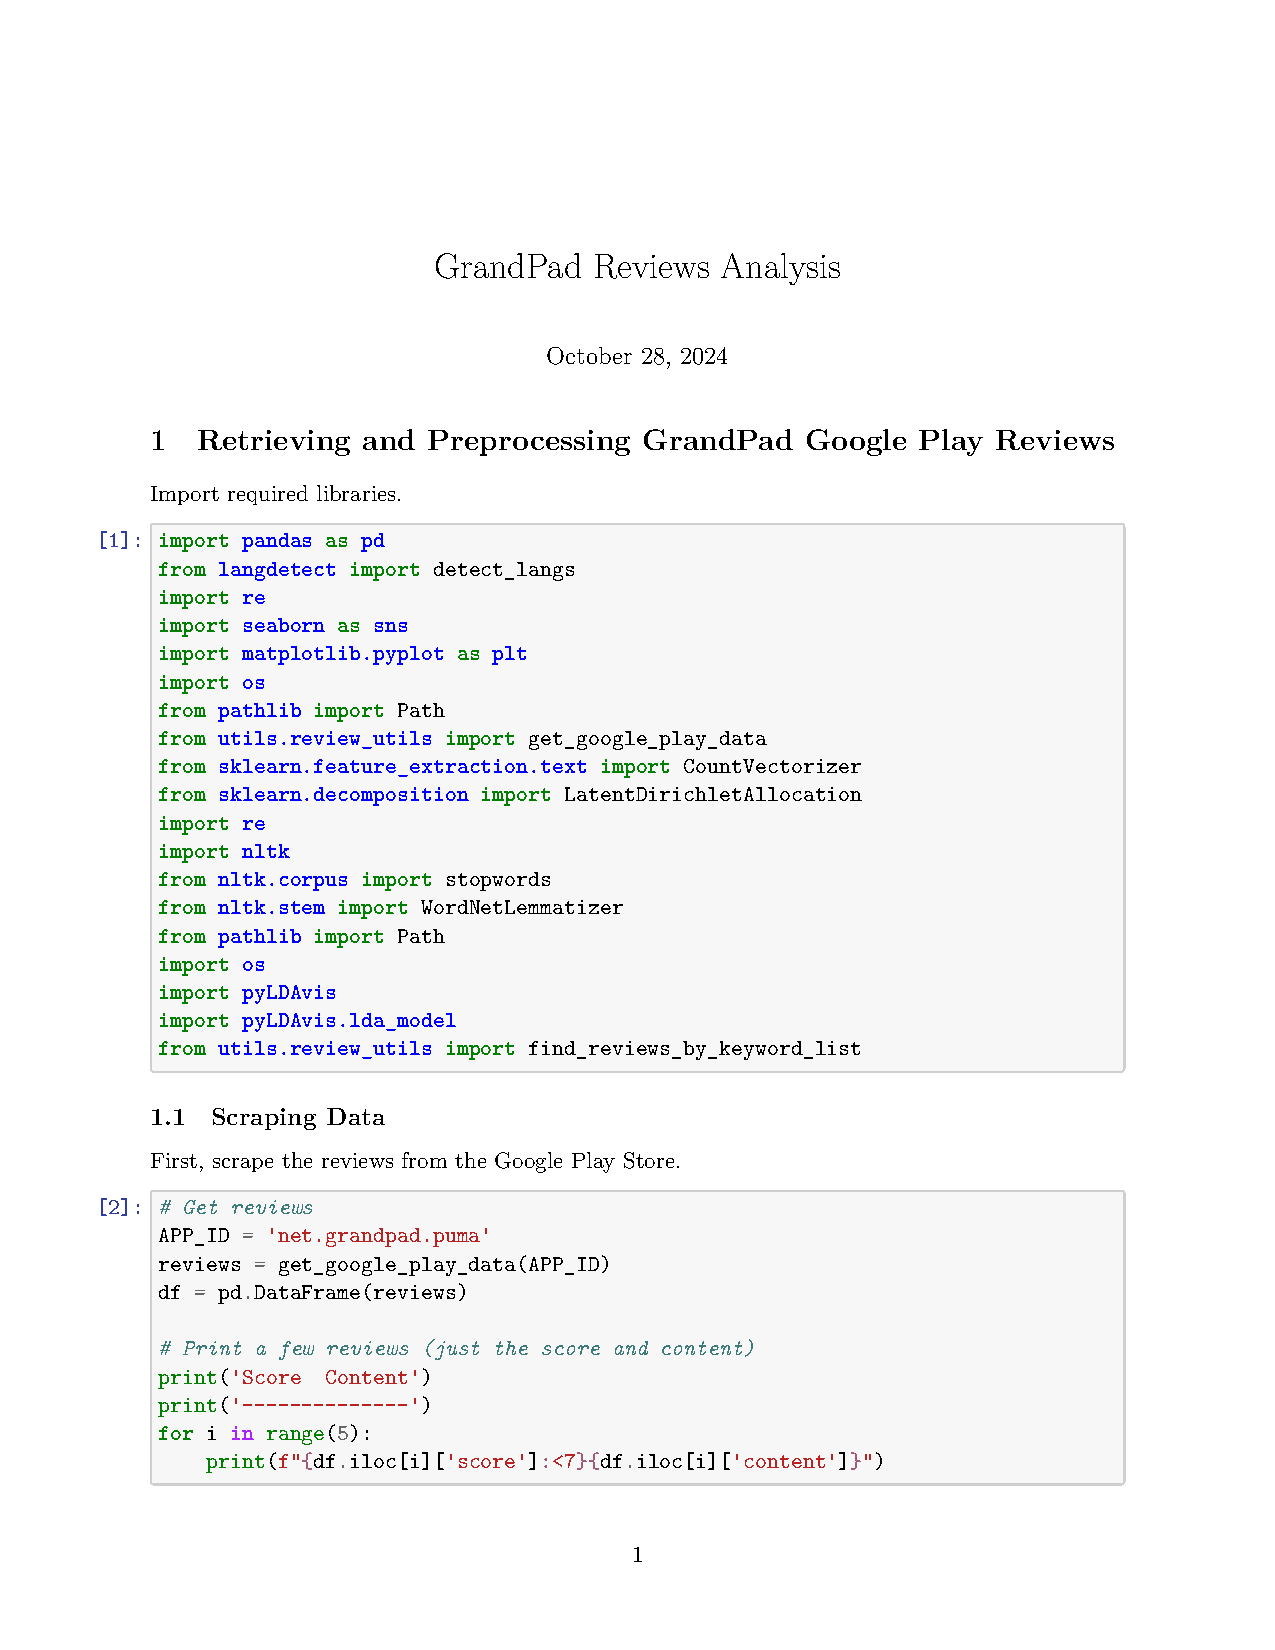
\includepdf[
                pages=-,
                width=\textwidth,
                pagecommand={\pagestyle{headings}},
                addtotoc={1,section,1,Jupyter Notebook: GrandPad Reviews Analysis,sec:reviews_processing_notebook}]
            {GrandPad Reviews Analysis.pdf}
        \end{appendices}

\end{document}
